\section{总变差}
\label{sec:dcomp-tv}

最直接的比较是逐个事件对照：同一个事件$A$，在一个分布下概率是$P(A)$，在另一个分布下是$Q(A)$。只要所有事件的概率差都小，用$Q$代替$P$去回答“某事发生的概率是多少”就不会出大错。把所有事件中最坏的那个差拿出来，就得到一个数。本节先给出这个数的定义和计算方法，再把它从事件推广到有界函数的平均。

全章设$P,Q$是同一个可测空间$(\mathcal{X},\mathcal{F}_{\mathcal{X}})$上的概率测度。$\mathcal{X}$可以是有限集、$\mathbb{R}^{d}$或其他取值空间，事件指$\mathcal{F}_{\mathcal{X}}$中的集合。

\subsection{定义与计算}
\label{sec:dcomp-tv-definition}

把每个事件上的概率差取绝对值，再在全体事件上取上确界，就得到总变差。

\begin{definition}[总变差]
\label{def:dcomp-tv}
$P$与$Q$之间的\term{总变差}（total variation distance）是
\begin{equation}
 d_{\mathrm{TV}}(P,Q)=\sup_{A\in\mathcal{F}_{\mathcal{X}}}\bigl\lvert P(A)-Q(A)\bigr\rvert .
 \label{eq:dcomp-tv-def}
\end{equation}
\end{definition}

由定义可以直接读出几条性质。每个概率差都在$[-1,1]$中，所以$0\leq d_{\mathrm{TV}}\leq1$。交换$P,Q$不改变绝对值，所以它对称。对第三个分布$R$与任一事件$A$，
\[
 \lvert P(A)-R(A)\rvert\leq\lvert P(A)-Q(A)\rvert+\lvert Q(A)-R(A)\rvert ,
\]
两边取上确界得到三角不等式。$d_{\mathrm{TV}}(P,Q)=0$表示每个事件的概率都相同，即$P=Q$。所以总变差是全体概率测度上的一个距离。

\paragraph{有限概率表}
先在章首的例子上计算。$\mathcal{X}=\{0,1,2\}$，两份概率表是
\[
 p=(0.6,\ 0.3,\ 0.1),\qquad q=(0.3,\ 0.3,\ 0.4) .
\]
下文称它为\emph{例表}。三个点有$8$个子集，逐个计算$P(A)-Q(A)$，结果列在表~\ref{tab:dcomp-tv-events}中。差最大的是$\{0\}$与$\{0,1\}$，都等于$0.3$；最小的是$\{2\}$与$\{1,2\}$，都等于$-0.3$。所以$d_{\mathrm{TV}}(P,Q)=0.3$。

\begin{BookInlineTable}
 \centering
 \caption{例表中每个事件的概率差。}
 \label{tab:dcomp-tv-events}
 \begin{tabular}{lcccccccc}
  \toprule
  $A$ & $\varnothing$ & $\{0\}$ & $\{1\}$ & $\{2\}$ & $\{0,1\}$ & $\{0,2\}$ & $\{1,2\}$ & $\mathcal{X}$\\
  \midrule
  $P(A)-Q(A)$ & $0$ & $0.3$ & $0$ & $-0.3$ & $0.3$ & $0$ & $-0.3$ & $0$\\
  \bottomrule
 \end{tabular}
\end{BookInlineTable}

表中有规律可循。事件的概率差是各点概率差之和，点$0$贡献$+0.3$，点$1$贡献$0$，点$2$贡献$-0.3$。要让和最大，就把所有贡献为正的点放进事件，把贡献为负的点排除在外，见图~\ref{fig:dcomp-tv-table}。最坏事件是$\{x:p(x)>q(x)\}$，最大的差等于正的差之和。又因为两表各自总和为$1$，正的差之和等于负的差之和的绝对值，各占全部绝对差的一半：
\[
 d_{\mathrm{TV}}(P,Q)=\tfrac12\bigl(\lvert0.3\rvert+\lvert0\rvert+\lvert-0.3\rvert\bigr)=0.3 .
\]

\begin{BookInlineFigure}
 \centering
 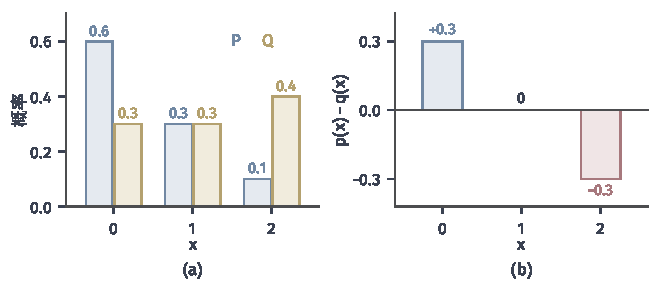
\includegraphics[width=112mm]{figures/07-probability/04-distribution-analysis/matplotlib/dcomp-tv-table/figure.pdf}
 \caption{例表的总变差。(a)蓝色柱为$P$，黄色柱为$Q$。(b)逐点概率差$p(x)-q(x)$，蓝色为正，红色为负。正的部分之和与负的部分之和的绝对值相等，都是$0.3$，即$d_{\mathrm{TV}}(P,Q)$。}
 \label{fig:dcomp-tv-table}
\end{BookInlineFigure}

\paragraph{共同支配测度}
要把这个规律推广到一般分布，需要一个能同时描述$P$与$Q$的“逐点概率”。有限表里它就是概率表本身；连续情形是密度；混有原子时两者都不够用。统一的办法是找一个测度$\lambda$，使$P,Q$都相对于它有密度。设$\lambda$是$\sigma$有限测度，并且$P\ll\lambda$，$Q\ll\lambda$，即$\lambda(A)=0$时$P(A)=Q(A)=0$。由Radon–Nikodym定理，存在非负可测函数$p,q$使
\begin{equation}
 P(A)=\int_{A}p\,\mathrm{d}\lambda,\qquad Q(A)=\int_{A}q\,\mathrm{d}\lambda,\qquad A\in\mathcal{F}_{\mathcal{X}},
 \label{eq:dcomp-common-density}
\end{equation}
并且$p,q$在$\lambda$几乎处处的意义下唯一，可参考\BookChapterRef{chap:measure-densities}{卷四第8章“测度的密度”}。这样的$\lambda$称为$P$与$Q$的\term{支配测度}（dominating measure），$p,q$称为它们相对于$\lambda$的密度。下文写$p,q$时，总是指相对于某个共同支配测度的密度。

支配测度总是存在：取$\lambda=P+Q$即可，因为$\lambda(A)=0$迫使$P(A)=Q(A)=0$。在有限表上$\lambda$取计数测度，$p,q$就是概率表；在$\mathbb{R}^{d}$上两者都有普通密度时，$\lambda$取Lebesgue测度。

\begin{theorem}[总变差的密度表示]
\label{thm:dcomp-tv-density}
设$p,q$是$P,Q$相对于共同支配测度$\lambda$的密度，$A^{*}=\{x:p(x)>q(x)\}$。则
\begin{equation}
 d_{\mathrm{TV}}(P,Q)=\frac12\int\lvert p-q\rvert\,\mathrm{d}\lambda=P(A^{*})-Q(A^{*})=1-\int\min(p,q)\,\mathrm{d}\lambda .
 \label{eq:dcomp-tv-density}
\end{equation}
\end{theorem}

\begin{proof}
先说明$A^{*}$达到上确界。对任一事件$A$，把它拆成$A\cap A^{*}$与$A\setminus A^{*}$。在$A^{*}$上$p-q>0$，在其外$p-q\leq0$，所以
\[
 P(A)-Q(A)=\int_{A}(p-q)\,\mathrm{d}\lambda\leq\int_{A\cap A^{*}}(p-q)\,\mathrm{d}\lambda\leq\int_{A^{*}}(p-q)\,\mathrm{d}\lambda .
\]
第一步丢掉了非正的部分，第二步补上了非负的部分。右端就是$P(A^{*})-Q(A^{*})$。同理，$Q(A)-P(A)\leq Q(B)-P(B)$，其中$B=(A^{*})^{\mathrm{c}}$。

再说明两个方向的最大值相等。两个密度的积分都是$1$，所以$\int(p-q)\,\mathrm{d}\lambda=0$，把积分拆到$A^{*}$与$B$上，得到
\[
 \int_{A^{*}}(p-q)\,\mathrm{d}\lambda=\int_{B}(q-p)\,\mathrm{d}\lambda .
\]
因此$\lvert P(A)-Q(A)\rvert$的上确界等于$P(A^{*})-Q(A^{*})$，即式~\eqref{eq:dcomp-tv-density}的第二个表达式。

$\lvert p-q\rvert$在$A^{*}$上等于$p-q$，在$B$上等于$q-p$。由上式，两部分积分相等，所以$\int\lvert p-q\rvert\,\mathrm{d}\lambda$是它们的两倍，这给出第一个表达式。最后，由$\lvert p-q\rvert=p+q-2\min(p,q)$，
\[
 \frac12\int\lvert p-q\rvert\,\mathrm{d}\lambda=\frac12\Bigl(1+1-2\int\min(p,q)\,\mathrm{d}\lambda\Bigr)=1-\int\min(p,q)\,\mathrm{d}\lambda .
\]
\end{proof}

式~\eqref{eq:dcomp-tv-density}的左端按定义~\eqref{eq:dcomp-tv-def}计算，与$\lambda$无关，所以右端也与支配测度的选取无关。最后一个表达式给出一个面积图景：$\int\min(p,q)\,\mathrm{d}\lambda$是两个密度的重叠部分，总变差是$1$减去重叠，也就是一个分布中“没有被另一个分布覆盖”的质量。

\paragraph{两个高斯分布}
取$P=\mathcal{N}(0,1)$，$Q=\mathcal{N}(1,1)$，以Lebesgue测度为支配测度。两个密度在$x=1/2$处相等，左侧$p>q$，所以$A^{*}=(-\infty,1/2)$。由式~\eqref{eq:dcomp-tv-density}，
\[
 d_{\mathrm{TV}}(P,Q)=\Phi\Bigl(\frac12\Bigr)-\Phi\Bigl(\frac12-1\Bigr)=2\Phi\Bigl(\frac12\Bigr)-1\approx0.3829 .
\]
图~\ref{fig:dcomp-tv-gaussians}(a)中浅蓝区域的面积是$\int(p-q)^{+}\,\mathrm{d}x$，浅黄区域是$\int(q-p)^{+}\,\mathrm{d}x$，两块面积相等，都是总变差。

\paragraph{没有共同普通密度的情形}
取
\[
 P=\operatorname{Unif}(0,1),\qquad Q=\tfrac12\operatorname{Unif}(0,1)+\tfrac12\delta_{1/2},
\]
即$Q$以一半概率均匀取值，另一半概率恰好取$1/2$。$Q$在单点$1/2$上有正概率，它没有Lebesgue密度。取$\lambda$为$(0,1)$上的Lebesgue测度加上$1/2$处的单位点质量，两个分布都被它支配，密度是
\[
 p(x)=\begin{cases}1,&x\in(0,1)\setminus\{\tfrac12\},\\0,&x=\tfrac12,\end{cases}\qquad
 q(x)=\begin{cases}\tfrac12,&x\in(0,1)\setminus\{\tfrac12\},\\\tfrac12,&x=\tfrac12 .\end{cases}
\]
在$x=1/2$处，$p$取$0$是因为$P(\{1/2\})=0$，而这一点上$\lambda$的质量是$1$，$q$必须等于$Q(\{1/2\})=1/2$。由式~\eqref{eq:dcomp-tv-density}，
\[
 d_{\mathrm{TV}}(P,Q)=\frac12\Bigl(\int_0^1\Bigl\lvert1-\frac12\Bigr\rvert\,\mathrm{d}x+\Bigl\lvert0-\frac12\Bigr\rvert\Bigr)=\frac12 .
\]
直接用定义检验：事件$\{1/2\}$的概率差就是$1/2$。图~\ref{fig:dcomp-tv-gaussians}(b)把原子画成竖线，它相对于$\lambda$的“密度”是该点的概率。

\begin{BookInlineFigure}
 \centering
 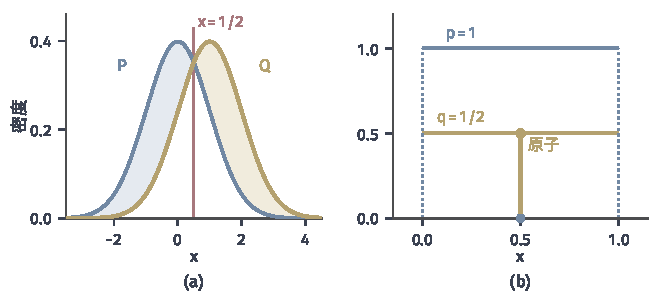
\includegraphics[width=112mm]{figures/07-probability/04-distribution-analysis/matplotlib/dcomp-tv-gaussians/figure.pdf}
 \caption{总变差的计算。(a)$P=\mathcal{N}(0,1)$（蓝）与$Q=\mathcal{N}(1,1)$（黄），红线是$x=1/2$；浅蓝区域$\{p>q\}$与浅黄区域$\{q>p\}$的面积都等于$d_{\mathrm{TV}}(P,Q)\approx0.3829$。(b)$P=\operatorname{Unif}(0,1)$（蓝）与$Q=\tfrac12\operatorname{Unif}(0,1)+\tfrac12\delta_{1/2}$（黄）相对于“Lebesgue测度加$1/2$处点质量”的密度；黄色竖线是$Q$在$1/2$处的原子，蓝点表示$P$在该点的密度为$0$。}
 \label{fig:dcomp-tv-gaussians}
\end{BookInlineFigure}

\paragraph{总变差看不到距离}
单点分布$\delta_x$与$\delta_y$（$x\neq y$）的总变差总是$1$：事件$\{x\}$在前者下概率为$1$，在后者下为$0$。无论$x,y$相距多近，结果都一样。更一般地，若存在事件$A$使$P(A)=1$，$Q(A)=0$，即$P$与$Q$相互奇异，则$d_{\mathrm{TV}}(P,Q)=1$，取到最大值。总变差只问“同一个事件的概率是否相同”，不问取值之间有多远。第~\ref{sec:dcomp-wasserstein}节会用位置移动的成本补上这个缺口。

\subsection{有界函数的期望差}
\label{sec:dcomp-tv-functions}

事件的概率是示性函数的期望：$P(A)=\mathbb{E}_{P}[\mathbf{1}_{A}]$。若关心的不是某件事是否发生，而是一个有界的数值结果，例如有上限的损失，那么要比较的是$\mathbb{E}_{P}[g]$与$\mathbb{E}_{Q}[g]$。总变差同样能控制它们，只是系数取决于$g$的取值范围。

\begin{theorem}[有界函数的期望差]
\label{thm:dcomp-tv-bounded}
设$g:\mathcal{X}\to\mathbb{R}$可测且有界，记$\operatorname{osc}(g)=\sup g-\inf g$。则
\begin{equation}
 \bigl\lvert\mathbb{E}_{P}[g]-\mathbb{E}_{Q}[g]\bigr\rvert\leq\operatorname{osc}(g)\,d_{\mathrm{TV}}(P,Q)\leq2\lVert g\rVert_{\infty}\,d_{\mathrm{TV}}(P,Q),
 \label{eq:dcomp-tv-osc}
\end{equation}
其中$\lVert g\rVert_{\infty}=\sup\lvert g\rvert$。并且
\begin{equation}
 \sup_{\lVert g\rVert_{\infty}\leq1}\bigl\lvert\mathbb{E}_{P}[g]-\mathbb{E}_{Q}[g]\bigr\rvert=2\,d_{\mathrm{TV}}(P,Q),
 \label{eq:dcomp-tv-dual}
\end{equation}
上确界在$g^{\pm}$处达到，$g^{\pm}$在$A^{*}$上取$1$，在其外取$-1$。
\end{theorem}

\begin{proof}
用共同支配测度写出期望差$\int g\,(p-q)\,\mathrm{d}\lambda$。因为$\int(p-q)\,\mathrm{d}\lambda=0$，被积函数中的$g$可以减去任意常数$c$而不改变积分：
\[
 \mathbb{E}_{P}[g]-\mathbb{E}_{Q}[g]=\int\bigl(g-c\bigr)(p-q)\,\mathrm{d}\lambda .
\]
取$c=(\sup g+\inf g)/2$，则$\lvert g-c\rvert\leq\operatorname{osc}(g)/2$处处成立。于是
\[
 \bigl\lvert\mathbb{E}_{P}[g]-\mathbb{E}_{Q}[g]\bigr\rvert\leq\frac{\operatorname{osc}(g)}{2}\int\lvert p-q\rvert\,\mathrm{d}\lambda=\operatorname{osc}(g)\,d_{\mathrm{TV}}(P,Q),
\]
最后一步用了式~\eqref{eq:dcomp-tv-density}。又$\operatorname{osc}(g)\leq2\lVert g\rVert_{\infty}$，得到式~\eqref{eq:dcomp-tv-osc}。

对$\lVert g\rVert_{\infty}\leq1$，上式给出期望差不超过$2d_{\mathrm{TV}}$。取$g=g^{\pm}$，则$g(p-q)=\lvert p-q\rvert$，期望差恰好是$\int\lvert p-q\rvert\,\mathrm{d}\lambda$，即$2d_{\mathrm{TV}}$，所以式~\eqref{eq:dcomp-tv-dual}的上确界达到。
\end{proof}

减去常数这一步是关键。概率差只对“质量怎样重新分配”敏感，整体平移$g$不影响结果，所以真正起作用的是$g$的振幅$\operatorname{osc}(g)$，而不是它的绝对大小。

\paragraph{系数的两种约定}
定义~\eqref{eq:dcomp-tv-def}在事件上取上确界，等价于在取值于$[0,1]$的函数上取上确界：这样的$g$满足$\operatorname{osc}(g)\leq1$，由式~\eqref{eq:dcomp-tv-osc}，期望差不超过$d_{\mathrm{TV}}$，而示性函数$\mathbf{1}_{A^{*}}$达到它。若改在单位球$\lVert g\rVert_{\infty}\leq1$上取上确界，函数可以从$-1$变到$1$，振幅加倍，结果是$2d_{\mathrm{TV}}$。有些文献把$\int\lvert p-q\rvert\,\mathrm{d}\lambda$称为总变差，它是本书$d_{\mathrm{TV}}$的两倍。读到“总变差小于$\varepsilon$”时，要先确认用的是哪一种约定。

\paragraph{例表上的检验}
在例表上取$g=g^{\pm}$。这里$A^{*}=\{0\}$，$g$在三个点上依次取$1,-1,-1$，两个期望是
\[
 \mathbb{E}_{P}[g]=0.6-0.3-0.1=0.2,\qquad\mathbb{E}_{Q}[g]=0.3-0.3-0.4=-0.4 .
\]
差为$0.6$，正是$2d_{\mathrm{TV}}$。再取$g(x)=x$，它的振幅是$2$，式~\eqref{eq:dcomp-tv-osc}给出的上界与实际的差分别是
\[
 2\times0.3=0.6,\qquad\lvert0.5-1.1\rvert=0.6,
\]
上界恰好达到。原因是$x=1-\tilde{g}(x)$，其中$\tilde{g}$在三点上依次取$1,0,-1$，而$\tilde{g}$正好在$p>q$处取最大值、在$p<q$处取最小值。一般的有界函数没有这样的巧合，上界会有余量。

式~\eqref{eq:dcomp-tv-dual}把总变差写成一类测试函数上的最大期望差。第~\ref{sec:dcomp-ipm}节会换用别的函数类得到别的比较量，第~\ref{sec:dcomp-expectation}节会把这个结果与其他比较量的类似结果放在一起，按评价函数的性质选择。
